% !TeX spellcheck = ru_RU
\documentclass[12pt, a4paper]{article}
\usepackage[a4paper, top=2cm, bottom=2cm, left=3cm, right=1cm]{geometry}
\usepackage[T2A]{fontenc}
\usepackage[utf8]{inputenc}
\usepackage[russian]{babel}
\usepackage{multirow}
\usepackage{listingsutf8}
\usepackage{float}
\usepackage{graphicx}
\usepackage{mathtools}
\usepackage{amsmath}
\mathtoolsset{showonlyrefs}
\usepackage{xcolor}
\usepackage{subfigure}



\definecolor{codegreen}{rgb}{0,0.6,0}
\definecolor{codegray}{rgb}{0.5,0.5,0.5}
\definecolor{codepurple}{rgb}{0.58,0,0.82}
\definecolor{backcolour}{rgb}{0.95,0.95,0.92}

\lstdefinestyle{mystyle}{
	backgroundcolor=\color{backcolour},   
	commentstyle=\color{codegreen},
	keywordstyle=\color{magenta},
	numberstyle=\tiny\color{codegray},
	stringstyle=\color{codepurple},
	basicstyle=\ttfamily\footnotesize,
	breakatwhitespace=false,         
	breaklines=true,                 
	captionpos=b,                    
	keepspaces=true,                 
	numbers=left,                    
	numbersep=5pt,                  
	showspaces=false,                
	showstringspaces=false,
	showtabs=false,                  
	tabsize=4
}

\lstset{inputencoding=utf8/koi8-r, style=mystyle}
\begin{document}
	
	\begin{titlepage}
		\centering{
			\MakeUppercase{\textbf{БЕЛОРУССКИЙ ГОСУДАРСТВЕННЫЙ УНИВЕРСИТЕТ}} \\[0.4cm]
			
			Факультет прикладной математики и информатики \\[0.4cm]
			
			\vspace{15em}
			
			{\large\bfseries{Отчёт по лабораторной работе №2}}
			
			{\large\bfseries{<<Интерполяция алгебраическими многочленами>>}} \\[4cm]
			
			\noindent
			\begin{tabular}{p{0.6\textwidth}p{0.6\textwidth}}
				& Выполнил: \\
				& Пищулёнок М.\,С. \\[1cm]
				& Преподаватель: \\
				& Горбачева Ю. Н.
				
			\end{tabular}
			
			\vfill
			
			{\normalsize Минск 2020}
			
		}
	\end{titlepage}
	
\tableofcontents
	
\section{Постановка задачи}
	
На отрезке $[a,b]$ заданы функции $f_1(x)$ и  $f_2(x)$. Построить многочлены степени $n =$ 3,  5,  7, 10, 15, интерполирующие каждую из них по узлам.
	
\begin{enumerate}
	\item равномерно расположены на указанном отрезке;
	\item расположенным на указанном отрезке оптимальным (минимизирующим погрешность) образом.
\end{enumerate}

\begin{align}
f_1(x) &= \sin(\cos x) & f_2(x) &= ||x| - 1|
\end{align}	

\section{Теория}

Разделённые разности определяются следующим образом:

\begin{equation}
	f(x_0, \ x_1, \ \dots  , x_{k+1}) = \frac{f(x_1, \ x_2, \ \dots, \ x_{k+1})-f(x_0, \ x_1, \ \dots, \ x_k)}{x_{k+1}- x_0}
	\label{eqn:razn}
\end{equation}

Будем использовать интерполяционный многочлен в форме Ньютона.

\begin{equation}
    P_n = f(x_0) + (x-x_0) f(x_0, x_1) + \dots + (x-x_0) \dots (x-x_{n-1}) f(x_0,  x_1, \dots, x_k)
    \label{eqn:newton_p}
\end{equation}

В качестве равномерно расположенных узлов, возьмём

\begin{equation}
	x_m = a + \frac{b-a}{n-1}m, \ \ m = 0, \ 1, \ \dots, \ n-1
	\label{eqn:ravn_rap}
\end{equation}

Для многочлена с минимальной погрешностью, в качестве узлов интерполирования возьмём корни многочлена Чебышёва после линейного преобразования $x = \frac{a+b}{2} - \frac{b-a}{2}t$

\begin{equation}
    x_m = \frac{b+a}{2} + \frac{b-a}{2} \cos \left( \frac{\pi (2m + 1)}{2n}\right), \, m = 0, \, 1, \, \dots, n-1.
    \label{eqn:cheb}
\end{equation}

Для оценки точности, будем использовать модуль остатка интерполирования:

\begin{equation}
	| r_n | = |f(x) - P_n(x)|
	\label{ost}
\end{equation}
	
\section{Программа}
	
\lstinputlisting[language=Python]{code/main.py}
	
\section{Результаты}

Для случаев 1, 2 найдем точки интерполирования (формулы \eqref{eqn:ravn_rap}, \eqref{eqn:cheb}). Вычислим разделённые разности (формула \eqref{eqn:razn}). Составим интерполирующие многочлены \eqref{eqn:newton_p}. Построим графики функции, многочленов, остатка интерполирования.

\begin{figure}[H]
	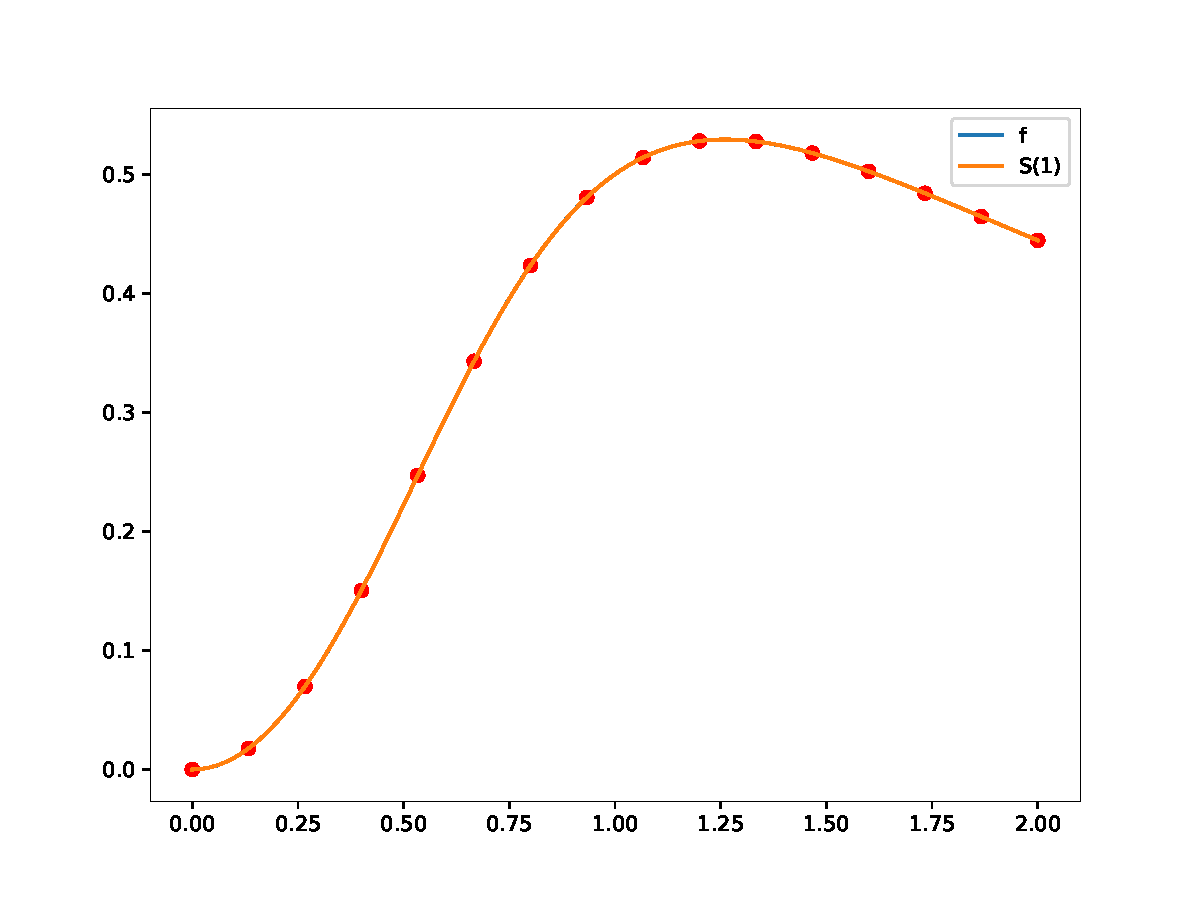
\includegraphics[width=0.5\linewidth]{images/1}
	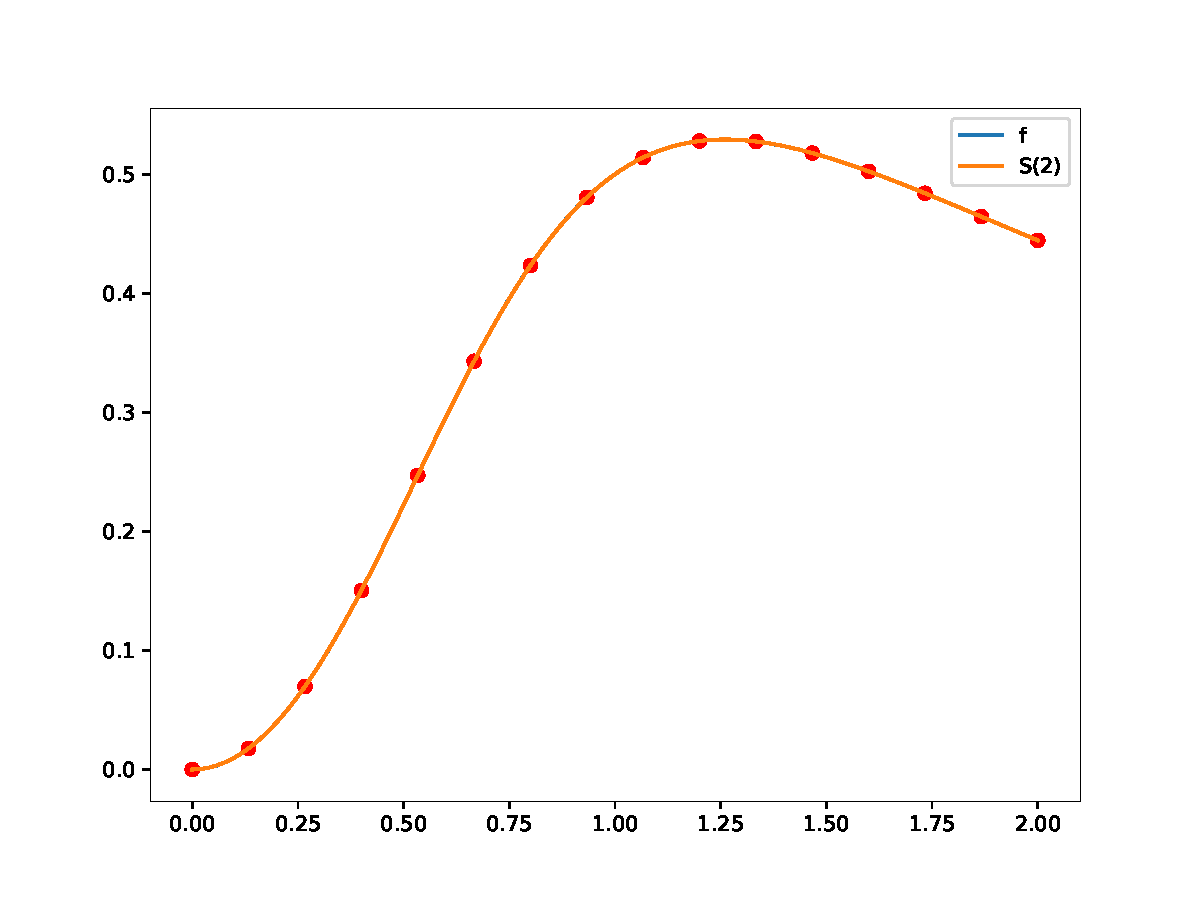
\includegraphics[width=0.5\linewidth]{images/2}
\end{figure}

\begin{figure}[H]
	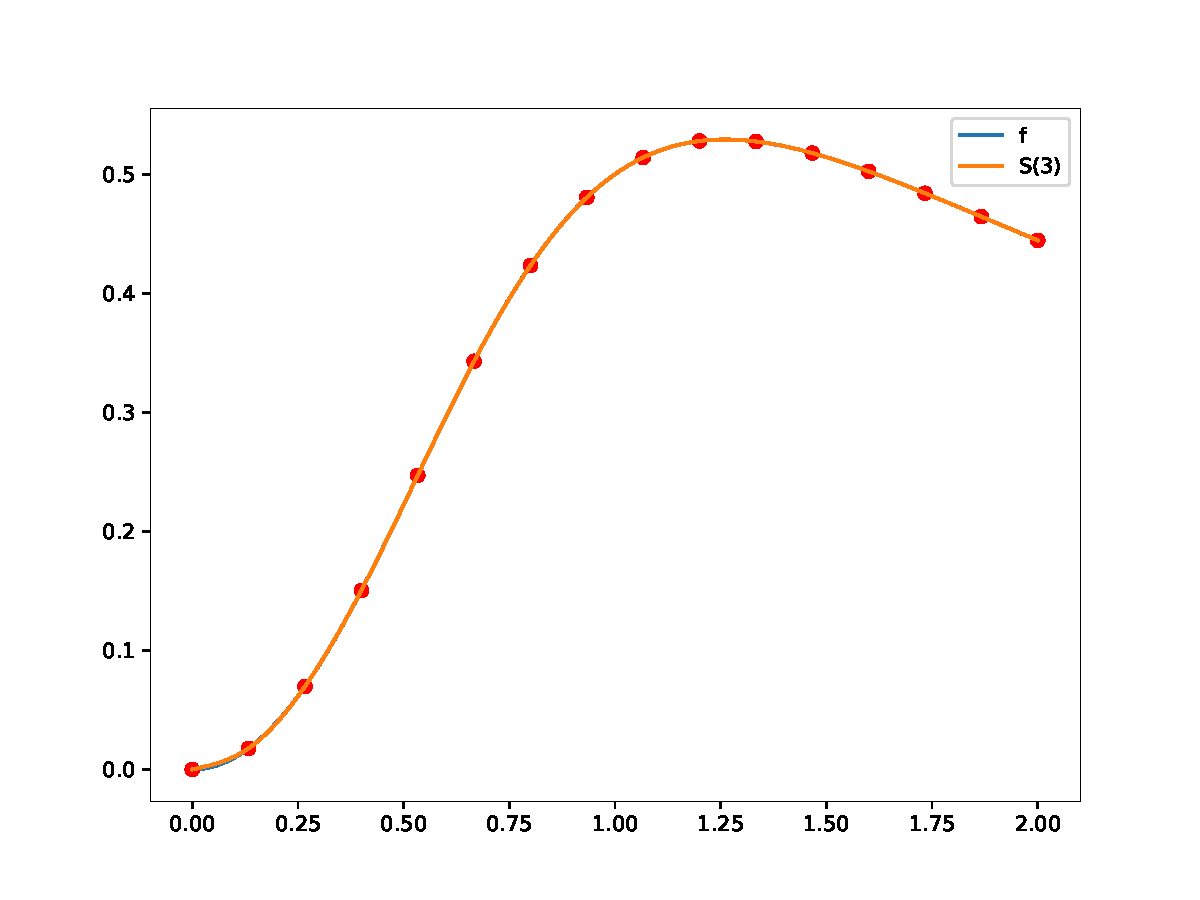
\includegraphics[width=0.5\linewidth]{images/3}
	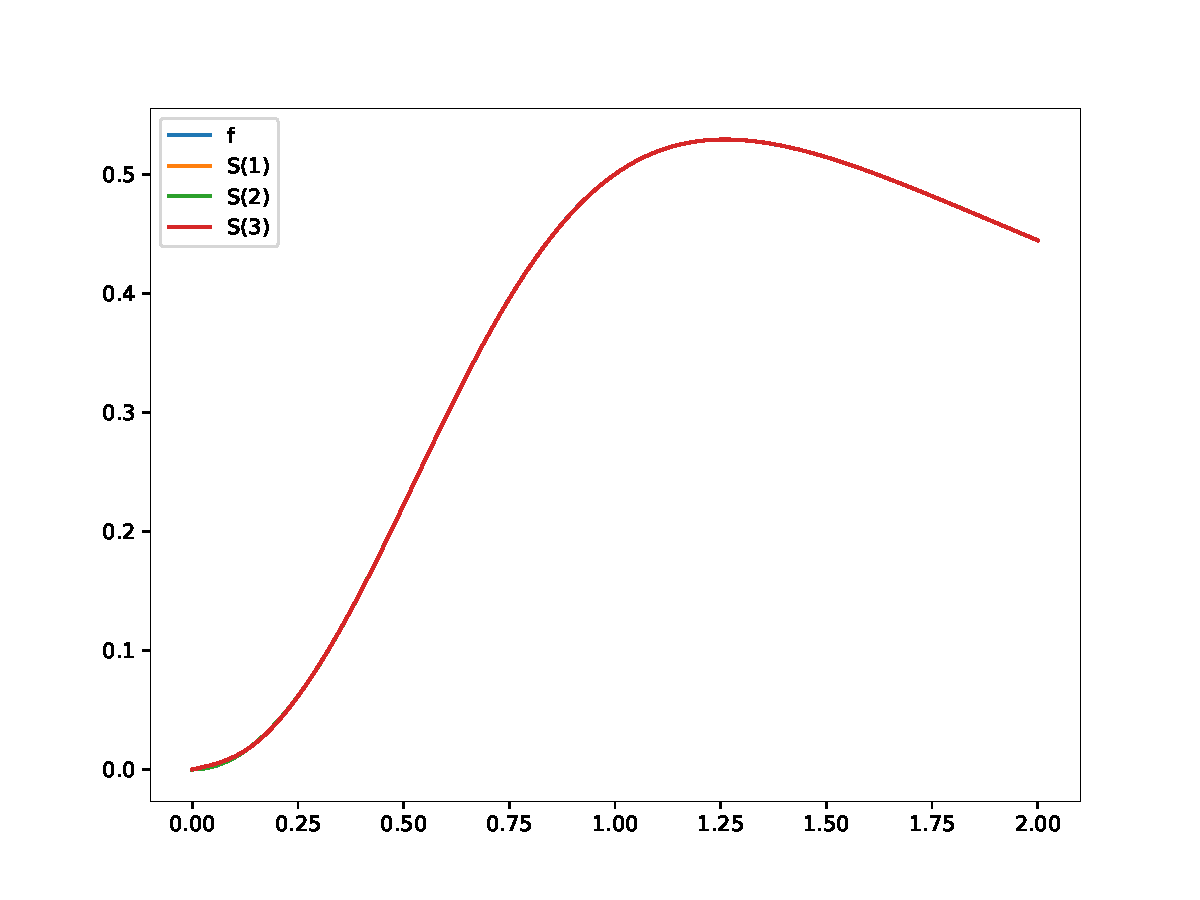
\includegraphics[width=0.5\linewidth]{images/4}
\end{figure}

\begin{figure}[H]
	\includegraphics[width=0.5\linewidth]{images/5}
	\includegraphics[width=0.5\linewidth]{images/6}
\end{figure}

\begin{figure}[H]
	\includegraphics[width=0.5\linewidth]{images/7}
	\includegraphics[width=0.5\linewidth]{images/8}
\end{figure}

\begin{figure}[H]
	\includegraphics[width=0.5\linewidth]{images/9}
	\includegraphics[width=0.5\linewidth]{images/10}
\end{figure}

\begin{figure}[H]
	\includegraphics[width=0.5\linewidth]{images/11}
	\includegraphics[width=0.5\linewidth]{images/12}
\end{figure}

\begin{figure}[H]
	\includegraphics[width=0.5\linewidth]{images/13}
	\includegraphics[width=0.5\linewidth]{images/14}
\end{figure}

\begin{figure}[H]
	\includegraphics[width=0.5\linewidth]{images/15}
	\includegraphics[width=0.5\linewidth]{images/16}
\end{figure}

\begin{figure}[H]
	\includegraphics[width=0.5\linewidth]{images/17}
	\includegraphics[width=0.5\linewidth]{images/18}
\end{figure}

\begin{figure}[H]
	\includegraphics[width=0.5\linewidth]{images/19}
	\includegraphics[width=0.5\linewidth]{images/20}
\end{figure}

\section{Выводы}
		
Один из способов уменьшить погрешность интерполяции -- выбор узлов. Если в качестве узлов интерполяции выбрать корни многочлена Чебышёва $\overline{T}_n^{[a,\ b]}(x)$, тогда 

\begin{equation}
	\max_{a \leq x \leq b}|\omega_{n+1}(x)| = (b-a)^{n+1}2^{1-2(n+1)}
	\label{eqn:max_pogr}
\end{equation}

При этом улучшить величину \eqref{eqn:max_pogr} уже нельзя.

\end{document}
